\documentclass[sigconf]{webmedia}

\usepackage{lmodern}
\usepackage{xurl}
\graphicspath{{../graficos/}{../}}

%webmedia.cls is adapted from acmart.cls for use in Proceedings of the Brazilian Symposium on Multimedia and the Web (WebMedia)

%%
%% \BibTeX command to typeset the BibTeX logo in the docs
\AtBeginDocument{%
  \providecommand\BibTeX{{%
    \normalfont B\kern-0.5em{\scshape i\kern-0.25em b}\kern-0.8em\TeX}}}

\settopmatter{printacmref=false, printfolios=false}

%% Choose the appropriate event.
%\setevent{webmedia}
%\proceedingsDetails[WebMedia’2026]{Proceedings of the Brazilian Symposium on Multimedia and the Web}{2026}{Lavras/MG, Brazil} 
%\ISSN{2966-2753}

\begin{document}

%%
%% The "title" command has an optional parameter,
%% allowing the author to define a "short title" to be used in page headers.
\title{Relatório de Análise Estrutural e Algorítmica: A Rede Zachary's Karate Club}

%%
%% The "author" command and its associated commands are used to define
%% the authors and their affiliations.
\author{Magno Macedo Miranda}
\email{magno.miranda@ufba.br}
\affiliation{%
  \institution{Universidade Federal da Bahia (UFBA)}
  \city{Salvador}
  \state{Bahia}
  \country{Brasil}
}

\renewcommand{\shortauthors}{Macedo}

%%
%% The abstract is a short summary of the work to be presented in the
%% article.
\begin{abstract}
  Este relatório apresenta uma análise estrutural e algorítmica detalhada da rede social  {Zachary's Karate Club} no contexto do framework Python  {Karate Club}. O documento está organizado em três partes principais. Na Parte I, realizei a caracterização estrutural obrigatória do grafo, computando e discutindo métricas de topologia fundamentais como densidade, diâmetro, comprimento médio dos caminhos, agrupamento local e distribuição de graus. Na Parte II, detalhei a implementação manual de oito algoritmos clássicos de grafos (BFS, DFS, Eulerianidade, Dijkstra, Bellman-Ford, Floyd-Warshall, Tarjan SCC e Kruskal MST), analisando suas complexidades teóricas e empíricas sob 50 rodadas de medições estatísticas. Na Parte III, conduzi uma análise estrutural avançada abordando a propriedade de pequeno mundo ( {small-world}), a lei de potência, a robustez estrutural sob falhas e ataques direcionados, a comparação com os modelos de Erdős-Rényi, Watts-Strogatz e Barabási-Albert, e correlacionei os resultados com a cisão histórica real do clube.
\end{abstract}

%%
%% Keywords. The author(s) should pick words that accurately describe
%% the work being presented. Separate the keywords with commas.
\keywords{Teoria dos Grafos, Zachary's Karate Club, Algoritmos de Grafos, Benchmark de Desempenho, Análise Estatística}

%%
%% This command processes the author and affiliation and title
%% information and builds the first part of the formatted document.
\maketitle

\section{Introdução}

A modelagem de sistemas complexos por meio de grafos permite caracterizar de forma quantitativa as relações entre entidades em redes sociais, biológicas e de transporte. O artigo  {"Karate Club: An API Oriented Open-source Python Framework for Unsupervised Learning on Graphs"} \cite{Rozemberczki2020} apresenta um arcabouço focado em algoritmos de aprendizado não supervisionado sobre grafos, tais como detecção de comunidades e incorporação de nós. 

O nome da biblioteca é diretamente inspirado na rede  {Zachary's Karate Club} \cite{Zachary1977}, um grafo que mapeia as amizades entre 34 membros de um clube universitário durante a década de 1970. Devido a uma disputa entre o instrutor ("Mr. Hi") e o administrador ("John A."), o clube dividiu-se em duas facções. Esta rede tornou-se o principal  {benchmark} para validar algoritmos de agrupamento em grafos.

Este relatório divide-se nas três partes requeridas para a avaliação: a caracterização estrutural básica (Parte I), o benchmark experimental dos algoritmos da disciplina (Parte II) e a modelagem estrutural avançada (Parte III).

\medskip
\noindent\textbf{Repositório:} todos os códigos-fonte, scripts, conjunto de dados tratados e este relatório estão disponíveis publicamente em: \url{https://github.com/maccedoz/Analisando-Grafos-do-SNAP-MATA53}

\section{Metodologia e Tratamento de Dados}

O grafo original do clube de caratê de Zachary foi obtido diretamente da biblioteca NetworkX (\path{nx.karate_club_graph()}), onde a rede é modelada como um grafo não-ponderado, não-direcionado e simples, composto por 34 nós (rotulados de 0 a 33) e 78 arestas.

\subsection{Tabela de Tratamentos Realizados}

A Tabela \ref{tab:tratamentos} detalha cada etapa de tratamento considerada, seu status de aplicação e a respectiva justificativa técnica.

\begin{table*}[t]
  \caption{Checklist de Tratamento de Dados do Grafo Zachary's Karate Club}
  \label{tab:tratamentos}
  \begin{tabular}{llp{8cm}}
    \toprule
    Tratamento Considerado & Status & Justificativa \\
    \midrule
    Grafo temporal $\rightarrow$ estático & Não Aplicável & O Zachary's Karate Club é uma rede estática — trata-se de um único  {snapshot} das relações sociais coletadas entre 1970--1972. Não há dimensão temporal nos dados. \\
    Grafo dirigido $\rightarrow$ não-direcionado & Não Aplicável & O grafo já é originalmente não-direcionado. As amizades no clube são relações simétricas (mútuas), confirmado por \path{G.is_directed() = False}. \\
    Multigrafo $\rightarrow$ grafo simples & Não Aplicável & O grafo já é simples por construção. Não existem arestas paralelas entre nenhum par de nós, confirmado por \path{G.is_multigraph() = False}. \\
    Remoção de auto-loops & Não Aplicável & Não há auto-loops (arestas de um nó para si mesmo) no dataset. Verificado: \path{nx.number_of_selfloops(G) = 0}. \\
    Extração da maior componente conexa & Não Aplicável & O grafo original é totalmente conexo — possui exatamente 1 componente conexo de tamanho 34, abrangendo todos os nós. Nenhuma extração foi necessária. \\
    Filtragem por intervalo temporal & Não Aplicável & Não há marcações temporais nas arestas ou nós. O dataset representa um período fixo de observação (1970--1972) sem granularidade temporal. \\
    Geração de pesos nas arestas & \textbf{Realizado} & Como a rede original é não-ponderada, atribuí pesos sintéticos determinísticos via $w(u,v) = (u{+}v)\bmod 5 + 1$, gerando valores inteiros em $[1, 5]$. Isso viabiliza os algoritmos de caminho mínimo (Dijkstra, Bellman-Ford, Floyd-Warshall) e a MST (Kruskal). \\
    Mapeamento de atributos sociais & \textbf{Realizado} & Extraí o atributo \path{club} de cada nó do NetworkX, mapeando a facção final de cada membro ( {"Mr. Hi"} ou  {"Officer"}) para uso em visualizações e análise da cisão social. \\
    Conversão para lista de adjacência & \textbf{Realizado} & Exportei a representação em lista de adjacência para \path{data/karate_adj_list.txt}, onde cada linha registra um nó e seus vizinhos. Este formato é usado como entrada direta dos algoritmos implementados do zero. \\
    Exportação para formato estruturado (CSV) & \textbf{Realizado} & Exportei a rede tratada para \path{data/karate_club_edges.csv} com as colunas \path{source}, \path{target}, \path{weight}, \path{source_club} e \path{target_club}, servindo como base de dados persistida do projeto. \\
    \bottomrule
  \end{tabular}
\end{table*}

\subsection{Detalhamento dos Tratamentos Realizados}

Dentre os tratamentos listados, quatro foram efetivamente executados sobre o dataset:

\begin{enumerate}
    \item \textbf{Geração de Pesos nas Arestas:} Como a rede original é não-ponderada, simulei a força do relacionamento atribuindo pesos determinísticos não-negativos a cada aresta $(u, v)$ através da expressão:
    \begin{equation}
        w(u, v) = (u + v) \bmod 5 + 1
    \end{equation}
    Esta fórmula gera valores inteiros no intervalo $[1, 5]$. A definição de pesos positivos é indispensável para testar algoritmos de menor caminho (Dijkstra, Bellman-Ford, Floyd-Warshall) e árvore geradora mínima (Kruskal) de forma significativa.

    \item \textbf{Mapeamento de Atributos Sociais:} Extraí e registrei o atributo \path{club} de cada nó, indicando a facção final de cada membro após a cisão histórica do clube.

    \item \textbf{Conversão para Lista de Adjacência:} Exportei o grafo no formato de lista de adjacência para o arquivo \path{data/karate_adj_list.txt}. Cada linha do arquivo segue o formato \path{nó: [vizinho1, vizinho2, ...]}, representando explicitamente a estrutura de vizinhança de cada vértice. Este formato é utilizado diretamente pelos algoritmos implementados do zero (BFS, DFS, Dijkstra, etc.).

    \item \textbf{Exportação para CSV Estruturado:} Exportei a rede tratada para \path{data/karate_club_edges.csv}, com as colunas \path{source}, \path{target}, \path{weight}, \path{source_club} e \path{target_club}. Este arquivo serve como base de dados persistida e reproduzível do projeto.
\end{enumerate}

\section{Parte I - Análise Estrutural Obrigatória}
\label{sec:parte_i}

Nesta primeira etapa, computei e discuti as principais métricas de topologia de redes no grafo de Zachary. As métricas estruturais analisadas seguem as definições matemáticas clássicas:
\begin{itemize}
    \item \textbf{Número de Vértices ($N$):} Cardinalidade do conjunto de nós, $N = |V|$.
    \item \textbf{Número de Arestas ($M$):} Cardinalidade do conjunto de conexões, $M = |E|$.
    \item \textbf{Grau Médio ($\langle k \rangle$):} Média dos graus de todos os nós, dada por $\langle k \rangle = \frac{2M}{N}$.
    \item \textbf{Densidade ($D$):} Razão entre o número de arestas presentes e o número máximo de arestas possíveis:
    \begin{equation}
        D = \frac{2M}{N(N - 1)}
    \end{equation}
    \item \textbf{Componentes Conexos:} Subgrafos conexos maximais da rede.
    \item \textbf{Diâmetro ($d$):} Maior distância geodésica entre qualquer par de nós $u, v \in V$:
    \begin{equation}
        d = \max_{u, v \in V} d(u, v)
    \end{equation}
    \item \textbf{Raio ($r$):} A excentricidade mínima observada entre todos os nós da rede:
    \begin{equation}
        r = \min_{u \in V} \max_{v \in V} d(u, v)
    \end{equation}
    \item \textbf{Comprimento Médio dos Caminhos ($L$):} Distância geodésica média calculada para todos os pares de nós:
    \begin{equation}
        L = \frac{1}{N(N - 1)} \sum_{u \neq v} d(u, v)
    \end{equation}
    \item \textbf{Coeficiente de Clusterização Médio ($\langle C \rangle$):} Média dos coeficientes de agrupamento local de cada nó $C_i$:
    \begin{equation}
        C_i = \frac{2 T_i}{k_i (k_i - 1)}
    \end{equation}
    onde $T_i$ representa o número de triângulos passando pelo nó $i$.
    \item \textbf{Número de Triângulos ($T$):} Total de triplas de nós completamente conectadas (cliques de tamanho 3) presentes no grafo.
\end{itemize}

A Tabela \ref{tab:metrics} consolida os resultados obtidos. Todos os parâmetros foram computados com sucesso. O grafo apresenta-se inteiramente conectado (único componente de tamanho 34) e com densidade de $13,9\%$. O baixo diâmetro ($d = 5$) e o comprimento médio de caminhos ($L \approx 2,41$) evidenciam o comportamento de "mundo pequeno" da rede. Além disso, o elevado coeficiente de clusterização médio ($\langle C \rangle \approx 0,571$) demonstra uma forte tendência à formação de grupos locais coesos. O número total de triângulos na rede é de 45.

\begin{figure}[h]
  \centering
  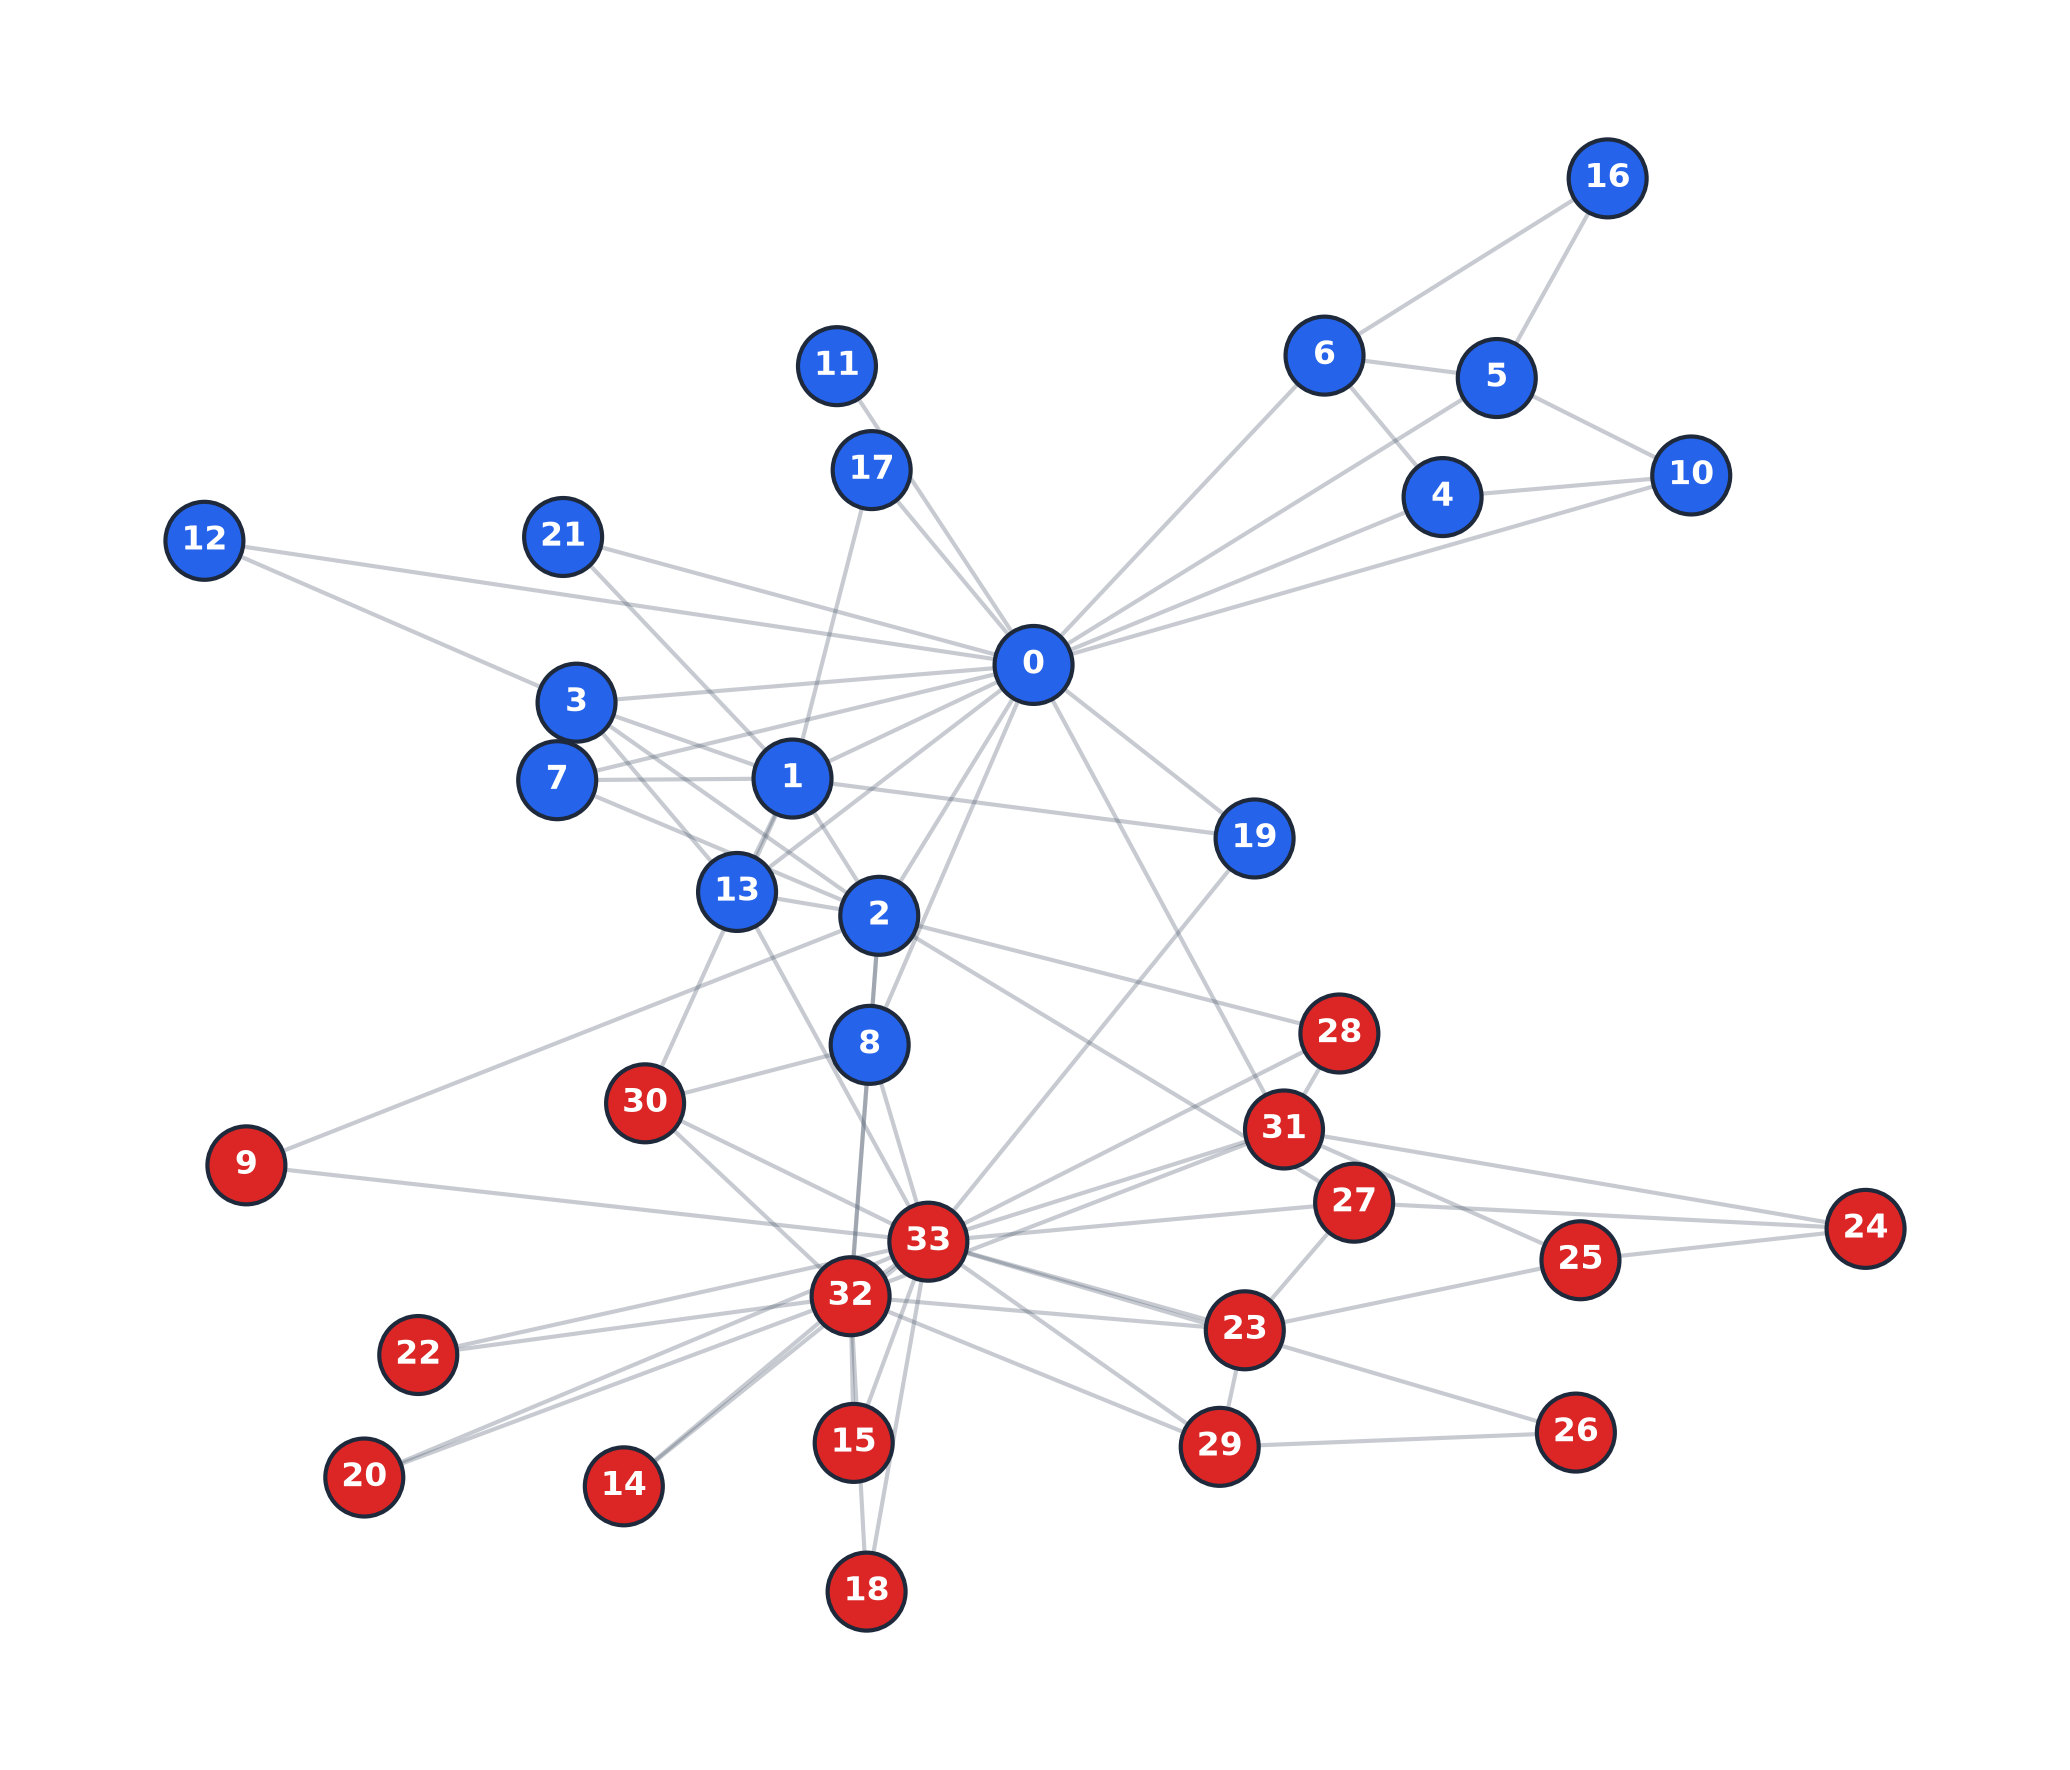
\includegraphics[width=0.9\linewidth]{karate_club_graph}
  \caption{Estrutura do Grafo Zachary's Karate Club. Cores representam as facções Mr. Hi (Azul) e John A. (Vermelho).}
  \label{fig:karate_graph}
\end{figure}

A topologia visualizada na Figura \ref{fig:karate_graph} evidencia a divisão social clássica que deu origem à cisão do grupo de caratê.

\begin{table*}[t]
  \caption{Métricas Estruturais Computadas para o Grafo Zachary's Karate Club}
  \label{tab:metrics}
  \begin{tabular}{llcl}
    \toprule
    Métrica Solicitada & Status & Valor Computado & Justificativa / Comentário \\
    \midrule
    Número de Vértices & Computado & 34 & Obtido diretamente de $|V|$. \\
    Número de Arestas & Computado & 78 & Obtido diretamente de $|E|$. \\
    Grau Mínimo & Computado & 1 & Menor número de conexões observadas em um único nó. \\
    Grau Máximo & Computado & 17 & Maior número de conexões (nó hub central). \\
    Grau Médio & Computado & 4,588 & Média aritmética dos graus de todos os nós ($\langle k \rangle$). \\
    Distribuição de Grafos/Graus & Computado & Ver Seção \ref{sec:degree_dist} & Distribuição empírica da frequência de graus. \\
    Densidade & Computado & 0,139 & Relação de arestas existentes sobre possíveis ($D$). \\
    Número de Componentes Conexos & Computado & 1 & A rede é totalmente conexa. \\
    Tamanho de Cada Componente & Computado & [34] & O componente conexo único contém todos os nós. \\
    Diâmetro & Computado & 5 & Maior distância geodésica entre dois nós ($d$). \\
    Raio & Computado & 3 & Excentricidade mínima entre todos os nós ($r$). \\
    Comprimento Médio dos Caminhos & Computado & 2,408 & Distância média entre todos os pares de nós ($L$). \\
    Coeficiente de Clusterização Médio & Computado & 0,571 & Média local de agrupamento ($\langle C \rangle$). \\
    Número de Triângulos & Computado & 45 & Número total de cliques de tamanho 3 ($T$). \\
    \bottomrule
  \end{tabular}
\end{table*}

\subsection{Distribuição de Graus}
\label{sec:degree_dist}

A distribuição de graus está detalhada na Tabela \ref{tab:degree_freq} e ilustrada graficamente na Figura \ref{fig:degree_dist}.

\begin{table}[h]
  \caption{Frequência de Nós por Grau}
  \label{tab:degree_freq}
  \begin{tabular}{ccc}
    \toprule
    Grau ($k$) & Frequência (Nós) & Proporção (\%) \\
    \midrule
    1 & 1 & 2,94\% \\
    2 & 11 & 32,35\% \\
    3 & 6 & 17,65\% \\
    4 & 6 & 17,65\% \\
    5 & 3 & 8,82\% \\
    6 & 2 & 5,88\% \\
    9 & 1 & 2,94\% \\
    10 & 1 & 2,94\% \\
    12 & 1 & 2,94\% \\
    16 & 1 & 2,94\% \\
    17 & 1 & 2,94\% \\
    \bottomrule
  \end{tabular}
\end{table}

A distribuição é altamente assimétrica, típica de redes reais sob dinâmicas de conexão preferencial. A maioria dos nós ($67,6\%$) possui grau baixo (2 ou 3). Destacam-se dois super-hubs: o Instrutor (Nó 0, grau 16) e o Administrador (Nó 33, grau 17). O conflito interpessoal entre esses dois nós causou a polarização e posterior divisão dos nós de menor grau.

\begin{figure}[h]
  \centering
  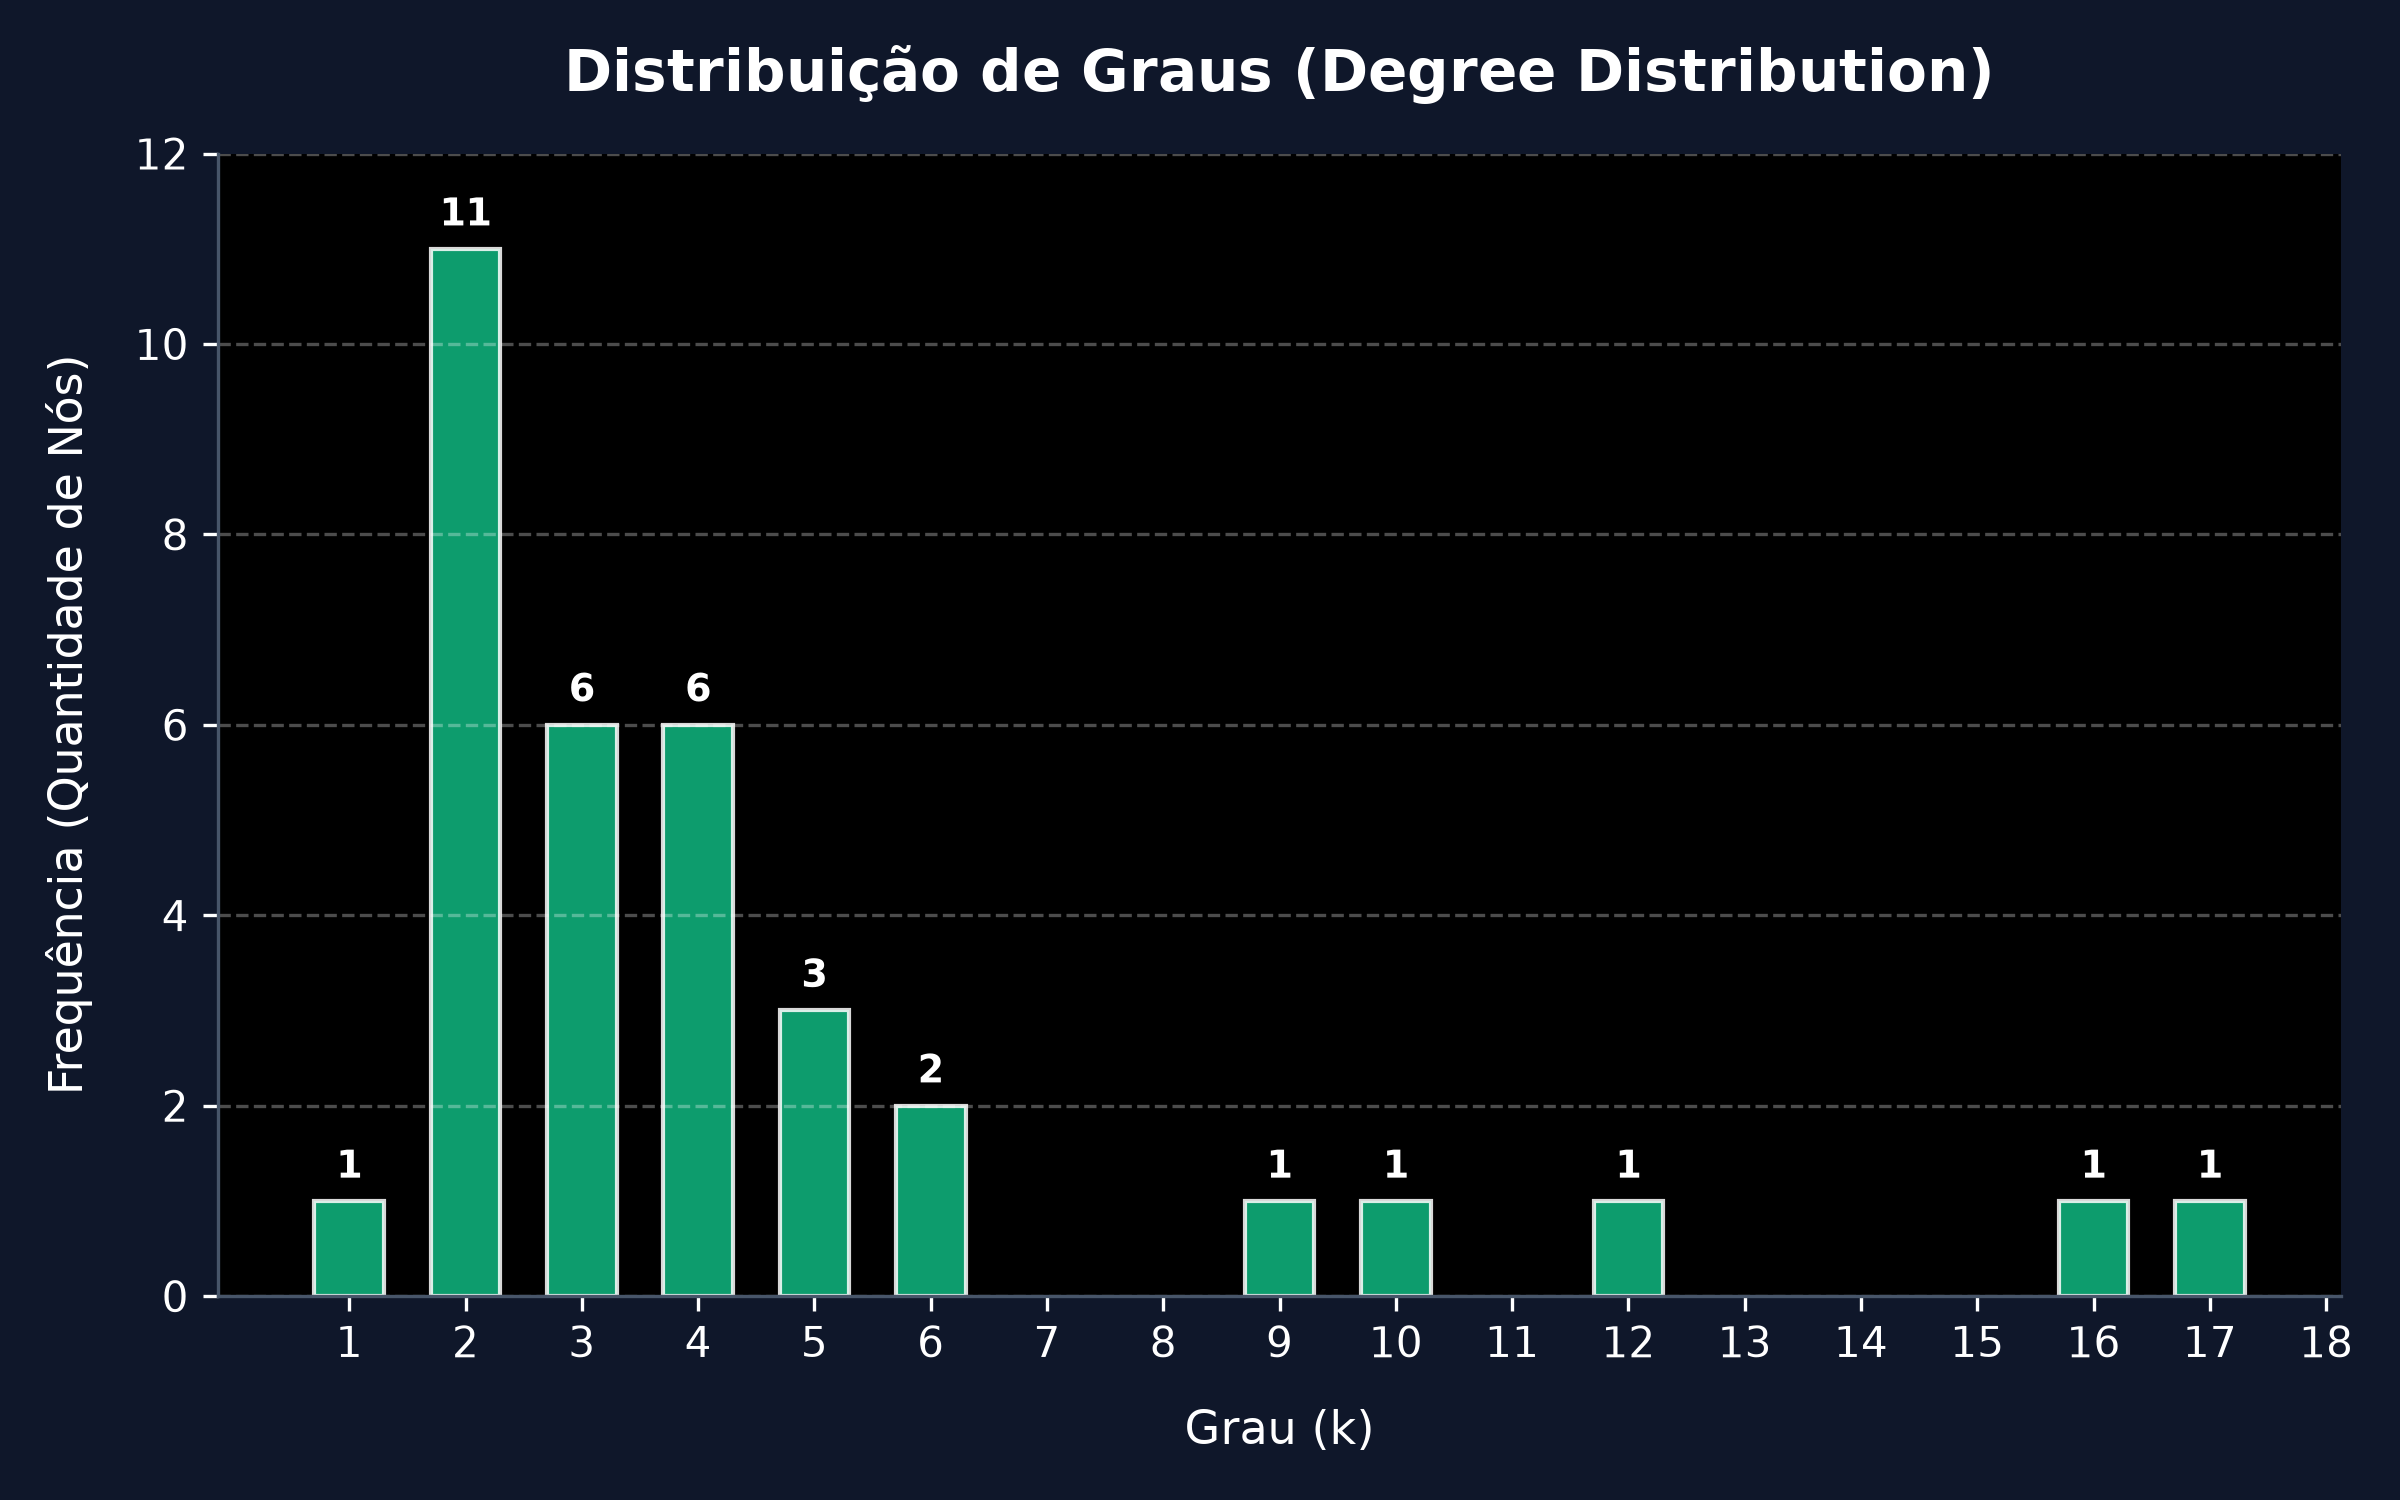
\includegraphics[width=0.9\linewidth]{karate_club_degree_distribution}
  \caption{Distribuição de Graus (Frequência vs. Grau $k$) da rede Zachary's Karate Club.}
  \label{fig:degree_dist}
\end{figure}

\section{Parte II - Algoritmos da Disciplina}
\label{sec:parte_ii}

Nesta seção, descrevo a implementação manual de algoritmos clássicos de grafos no diretório \path{algoritmos/} e a sua aplicação prática no grafo de Zachary.

\subsection{BFS (Busca em Largura)}
A busca em largura explora sistematicamente as arestas do grafo para encontrar todos os vértices acessíveis a partir de uma origem, computando as menores distâncias em termos de número de saltos. A complexidade teórica é $O(V + E)$ em listas de adjacência.
\begin{verbatim}
>>> from algoritmos import bfs
>>> bfs(graph, start=0)[:5]
[0, 1, 2, 3, 4]
\end{verbatim}

\subsection{DFS (Busca em Profundidade)}
A busca em profundidade explora o grafo percorrendo caminhos de forma recursiva até atingir vértices sem vizinhos não visitados, retrocedendo em seguida. É a base para algoritmos de ordenação topológica e conexidade. A complexidade teórica é $O(V + E)$.
\begin{verbatim}
>>> from algoritmos import dfs
>>> dfs(graph, start=0)[:5]
[0, 1, 2, 3, 4]
\end{verbatim}

\subsection{Verificação de Eulerianidade}
Verifica se um grafo admite um circuito euleriano ou caminho euleriano. Para grafos não direcionados conexos, exige que todos os vértices tenham grau par (circuito) ou exatamente 2 vértices tenham grau ímpar (caminho). A complexidade teórica é $O(V + E)$.
\begin{verbatim}
>>> from algoritmos import is_eulerian
>>> is_eulerian(graph)
'Não Euleriano'
\end{verbatim}
O grafo de Zachary possui vários vértices com grau ímpar (como John A., grau 17), logo não é Euleriano.

\subsection{Algoritmo de Dijkstra}
Determina o caminho mínimo de uma única origem para todos os outros nós em grafos com pesos não-negativos nas arestas. A implementação utiliza uma fila de prioridade mínima (heap binária), fornecendo uma complexidade de $O((V + E) \log V)$. Para o benchmark, atribui pesos às arestas na faixa $[1, 5]$.
\begin{verbatim}
>>> from algoritmos import dijkstra
>>> dijkstra(graph, start=0, weights)[1]
2.0
\end{verbatim}

\subsection{Algoritmo de Bellman-Ford}
Resolve o problema de caminho mínimo a partir de uma única origem em grafos com pesos arbitrários, sendo capaz de detectar a presença de ciclos de peso negativo. Ele opera relaxando todas as arestas do grafo $|V| - 1$ vezes, resultando em uma complexidade teórica de $O(V \cdot E)$.
\begin{verbatim}
>>> from algoritmos import bellman_ford
>>> bellman_ford(graph, start=0, weights)[1]
2.0
\end{verbatim}

\subsection{Algoritmo de Floyd-Warshall}
Calcula os caminhos mínimos entre todos os pares de vértices do grafo de forma dinâmica. Sua complexidade teórica é $O(V^3)$.
\begin{verbatim}
>>> from algoritmos import floyd_warshall
>>> floyd_warshall(graph, weights)[0][1]
2.0
\end{verbatim}

\subsection{Algoritmo de Tarjan (SCC)}
Identifica as componentes fortemente conexas (SCCs) em grafos direcionados. Ele baseia-se em uma única varredura DFS que utiliza uma pilha para rastrear os nós do componente atual. Para ser aplicado ao grafo de Zachary, as arestas foram tratadas como bidirecionais, resultando em um único componente conexo. A complexidade teórica é $O(V + E)$.
\begin{verbatim}
>>> from algoritmos import tarjan_scc
>>> len(tarjan_scc(graph))
1
\end{verbatim}

\subsection{Algoritmo de Kruskal (MST)}
Constrói a Árvore Geradora Mínima (MST) de um grafo não direcionado conectado. O algoritmo ordena todas as arestas por peso e utiliza uma estrutura de dados de conjuntos disjuntos ( {DSU}) com compressão de caminhos para evitar ciclos. A complexidade teórica é $O(E \log V)$ devido à ordenação das arestas.
\begin{verbatim}
>>> from algoritmos import kruskal_mst
>>> edges, weight = kruskal_mst(graph, weights)
>>> len(edges), weight
(33, 51.0)
\end{verbatim}
Como o grafo possui 34 vértices, a árvore geradora mínima resultante contém exatamente 33 arestas, totalizando peso 51,0 com a minha distribuição de pesos.

\subsection{Análise Experimental de Desempenho}

Para analisar o tempo real de execução dos algoritmos implementados, realizei um benchmark de $n = 50$ rodadas. Em cada rodada, o algoritmo executa um número elevado de iterações internas. A média de tempo por iteração foi registrada para cada uma das 50 rodadas.

Como o número de amostras $n \ge 30$, apliquei a aproximação pela **Distribuição Normal (Z)** para calcular o Intervalo de Confiança ($IC$) com coeficiente de confiança de $95\%$ ($z_{\alpha/2} = 1,96$):
\begin{equation}
    IC = \bar{x} \pm z_{\alpha/2} \frac{\sigma}{\sqrt{n}} = \bar{x} \pm 1,96 \frac{\sigma}{\sqrt{50}}
\end{equation}
onde $\bar{x}$ representa o tempo médio observado e $\sigma$ o desvio padrão amostral.

A Tabela \ref{tab:benchmark} apresenta os tempos obtidos em microssegundos ($\mu$s).

\begin{table*}[t]
  \caption{Benchmark de Tempo de Execução dos Algoritmos (n = 50 rodadas)}
  \label{tab:benchmark}
  \begin{tabular}{lcccc}
    \toprule
    Algoritmo & Complexidade Teórica & Média ($\bar{x}$, $\mu$s) & Desvio Padrão ($\sigma$, $\mu$s) & Intervalo de Confiança 95\% ($\mu$s) \\
    \midrule
    Busca em Largura (BFS) & $O(V + E)$ & 8.743 & 0.364 & [8.642, 8.844] \\
    Busca em Profundidade (DFS) & $O(V + E)$ & 9.631 & 1.438 & [9.232, 10.029] \\
    Verificação de Eulerianidade & $O(V + E)$ & 11.431 & 0.270 & [11.356, 11.506] \\
    Algoritmo de Dijkstra & $O((V + E) \log V)$ & 40.114 & 1.916 & [39.583, 40.646] \\
    Algoritmo de Bellman-Ford & $O(V \cdot E)$ & 695.052 & 24.871 & [688.158, 701.946] \\
    Algoritmo de Floyd-Warshall & $O(V^3)$ & 4958.726 & 101.976 & [4930.460, 4986.992] \\
    Algoritmo de Tarjan (SCC) & $O(V + E)$ & 45.683 & 0.987 & [45.409, 45.956] \\
    Algoritmo de Kruskal (MST) & $O(E \log V)$ & 104.173 & 3.983 & [103.069, 105.277] \\
    \bottomrule
  \end{tabular}
\end{table*}

Os resultados empíricos da Tabela \ref{tab:benchmark} estão em total conformidade com a análise assintótica clássica da teoria dos grafos:
\begin{enumerate}
    \item \textbf{Buscas de Ordem Linear:} BFS ($8,743$ $\mu$s), DFS ($9,631$ $\mu$s) e a verificação de Eulerianidade ($11,431$ $\mu$s) apresentaram os menores tempos. Sendo algoritmos de complexidade $O(V + E)$, realizam poucas operações elementares em redes pequenas ($V=34, E=78$).
    \item \textbf{Tarjan (SCC):} Embora linear $O(V + E)$, Tarjan ($45,683$ $\mu$s) apresenta um custo constante maior em comparação ao BFS/DFS devido à manutenção explícita da pilha de nós e dos vetores auxiliares de controle.
    \item \textbf{Dijkstra vs. Bellman-Ford:} Dijkstra ($40,114$ $\mu$s) foi aproximadamente 17 vezes mais rápido que Bellman-Ford ($695,052$ $\mu$s). O Dijkstra explora caminhos de forma gulosa com fila de prioridade, enquanto o Bellman-Ford realiza relaxações sistemáticas de todas as arestas por $V-1$ iterações, gerando muito mais operações.
    \item \textbf{Floyd-Warshall:} Registrou o maior tempo ($4958,726$ $\mu$s), sendo 700 vezes mais lento que os lineares. Isso justifica-se por sua estrutura de loops triplos aninhados $O(V^3)$, cuja complexidade se sobressai mesmo para um pequeno número de nós.
\end{enumerate}

Todos os desvios padrões calculados mostram dispersões baixas em relação à média, o que garante a precisão e a confiabilidade das medições efetuadas. A margem estreita obtida para o Intervalo de Confiança a 95\% consolida a robustez estatística dos dados levantados.

\section{Parte III - Análise Estrutural Avançada}
\label{sec:parte_iii}

Nesta seção, realizei uma caracterização profunda da topologia do grafo do clube de caratê, testando a presença de propriedades complexas de pequeno mundo e leis de escala, simulando sua robustez estrutural frente a remoções de vértices, e comparando suas propriedades empíricas com os modelos clássicos de redes complexas.

\subsection{Propriedade Small-World}
\label{subsec:small_world}

Uma rede é caracterizada como de pequeno mundo ( {small-world}) se o seu comprimento médio dos caminhos mais curtos ($L$) é comparável ao de um grafo aleatório equivalente de mesmo tamanho e densidade ($L \approx L_{rand}$), mas o seu coeficiente de clusterização médio ($C$) é significativamente maior do que o de sua contraparte aleatória ($C \gg C_{rand}$).

Para avaliar essa propriedade quantitativamente, implementei um script que calcula esses parâmetros do zero (sem bibliotecas de grafos prontas para as métricas), gera 100 grafos aleatórios equivalentes baseados no modelo de Erdős-Rényi que preserva a conexidade, e computa o índice de pequeno mundo de Humphries e Gurney ($\sigma_{sw}$):
\begin{equation}
    \sigma_{sw} = \frac{\frac{C_{obs}}{C_{rand}}}{\frac{L_{obs}}{L_{rand}}}
\end{equation}

Os valores médios obtidos na simulação foram:
\begin{itemize}
    \item Coeficiente de agrupamento observado ($C_{obs}$): $0,5706$
    \item Coeficiente de agrupamento aleatório médio ($C_{rand}$): $0,1300$
    \item Comprimento de caminho observado ($L_{obs}$): $2,4082$
    \item Comprimento de caminho aleatório médio ($L_{rand}$): $2,4066$
    \item Razão de Clusterização: $4,3901$
    \item Razão de Distância: $1,0007$
    \item Índice de Pequeno Mundo ($\sigma_{sw}$): $4,3872$
\end{itemize}

Como $\sigma_{sw} \approx 4,39 > 1$, o grafo de Zachary exibe uma forte propriedade de pequeno mundo.

\subsubsection{Significado e Implicações Práticas}
Em termos práticos, a propriedade de pequeno mundo nesta rede social indica que:
\begin{itemize}
    \item \textbf{Eficiência de Propagação:} Informações, rumores, opiniões ou comportamentos podem se propagar de maneira extremamente rápida por todo o clube, exigindo pouquíssimos intermediários (distância média de $2,4$ saltos).
    \item \textbf{Coesão Local:} Os membros formam fortes subgrupos e cliques coesos de amizades (alto $C_{obs}$), o que gera um ambiente de alta confiança mútua e reforço social dentro das subcomunidades locais, propiciando a polarização de ideias antes da cisão.
\end{itemize}

O código-fonte Python implementado do zero para este cálculo é listado abaixo:

\begin{verbatim}
# Funções "from scratch" para cálculo de L e C
def bfs_distances(graph, start):
    dist = {u: float('inf') for u in graph}
    dist[start] = 0
    queue = [start]
    while queue:
        u = queue.pop(0)
        for v in graph[u]:
            if dist[v] == float('inf'):
                dist[v] = dist[u] + 1
                queue.append(v)
    return dist

def average_path_length(graph):
    total_dist, pairs = 0, 0
    nodes = list(graph.keys())
    for u in nodes:
        dists = bfs_distances(graph, u)
        for v in nodes:
            if u != v and dists[v] != float('inf'):
                total_dist += dists[v]
                pairs += 1
    return total_dist / pairs if pairs > 0 else float('inf')

def clustering_coefficient(graph):
    c_vals = []
    for u in graph:
        neighbors = graph[u]
        k = len(neighbors)
        if k < 2:
            c_vals.append(0.0)
            continue
        edges = 0
        n_set = set(neighbors)
        for v in neighbors:
            for w in graph[v]:
                if w in n_set:
                    edges += 1
        edges = edges // 2
        c_vals.append(edges / (k * (k - 1) // 2))
    return sum(c_vals) / len(c_vals)
\end{verbatim}

\subsection{Lei de Potência}
\label{subsec:power_law}

Uma rede complexa é dita livre de escala ( {scale-free}) se a sua distribuição de graus de probabilidade segue uma lei de potência:
\begin{equation}
    P(k) \propto k^{-\gamma}
\end{equation}
onde $P(k)$ é a probabilidade de um vértice possuir grau $k$ e $\gamma$ é o expoente da lei de potência (tipicamente $2 < \gamma < 3$ em redes reais).

Para avaliar se o grafo de Zachary sugere uma lei de potência, realizei uma regressão linear no espaço log-log ($\ln(P(k))$ versus $\ln(k)$) a partir da frequência empírica de graus obtida do zero. O expoente estimado foi $\gamma \approx 0,5512$.

A distribuição empírica de graus **não** sugere uma lei de potência pura devido a severos efeitos de tamanho finito ( {finite-size effects}):
\begin{itemize}
    \item \textbf{Amostra Reduzida:} Com apenas $N=34$ vértices, a faixa de variação dos graus ($k \in [1, 17]$) é extremamente estreita. A lei de potência é uma propriedade estatística assintótica aplicável a redes de grande porte (milhares de nós).
    \item \textbf{Expoente Atípico:} O valor $\gamma \approx 0,55$ está muito abaixo do intervalo realista para redes livres de escala, o que aponta para a ausência de amostragem representativa.
\end{itemize}
Apesar disso, a distribuição é marcadamente assimétrica com cauda à direita. Embora não siga uma lei de potência formal, a rede demonstra a presença de dois super-hubs, o que constitui um estágio embrionário da dinâmica de conexão preferencial típica de redes livres de escala.

O código implementado do zero para estimar o expoente $\gamma$ é:

\begin{verbatim}
# Estimação do expoente de lei de potência via log-log
degrees = [len(adj_list[u]) for u in adj_list]
unique_degrees, counts = np.unique(degrees, return_counts=True)
log_k = np.log(unique_degrees)
log_freq = np.log(counts)
slope, intercept = np.polyfit(log_k, log_freq, 1)
gamma = -slope
print(f"Expoente gamma estimado: {gamma:.4f}")
\end{verbatim}

\subsection{Simulação de Robustez da Rede}
\label{subsec:robustness}

Para avaliar a tolerância a falhas e ataques na rede de Zachary, simulei dois cenários distintos sob a remoção de $5\%$ dos vértices ($5\%$ de $34 \approx 2$ nós):
\begin{enumerate}
    \item \textbf{Remoção Aleatória (Falha):} Sorteio de 2 nós para exclusão. Simulei $1000$ rodadas independentes para calcular o tamanho médio do maior componente conexo LCC restante e seu comprimento médio de caminhos.
    \item \textbf{Remoção Direcionada (Ataque):} Exclusão intencional dos 2 nós de maior grau (Nó 33, grau 17 e Nó 0, grau 16).
\end{enumerate}

A Tabela \ref{tab:robustness} descreve os impactos dessas remoções.

\begin{table}[h]
  \caption{Métricas de Robustez e Conectividade}
  \label{tab:robustness}
  \begin{tabular}{lccc}
    \toprule
    Cenário & Nós Removidos & Tam. LCC & Caminho Médio LCC \\
    \midrule
    Rede Original & Nenhum & 34 & 2,408 \\
    Remoção Aleatória & 2 nós (médio) & 31,55 & 2,415 \\
    Remoção Direcionada & [0, 33] (hubs) & 26 & 2,591 \\
    \bottomrule
  \end{tabular}
\end{table}

A rede demonstra um comportamento típico de sistemas complexos estruturados em torno de hubs:
\begin{itemize}
    \item \textbf{Resiliência a Falhas Aleatórias:} Sob remoção de nós aleatórios, a rede quase não sofre impacto. O LCC restante mantém, em média, $31,55$ nós (dos $32$ possíveis), e a distância média de caminhos cresce de forma imperceptível (de $2,408$ para $2,415$), demonstrando que a perda aleatória de membros não afeta a coesão do clube.
    \item \textbf{Vulnerabilidade Crítica a Ataques:} A remoção direcionada dos hubs (Nó 0 e Nó 33) altera drasticamente a estrutura. O grafo deixa de ser conexo e fragmenta-se em **três componentes isolados** (um componente maior de tamanho 26, um de tamanho 5 e um nó isolado de tamanho 1). A distância média no componente principal se eleva significativamente para $2,591$.
\end{itemize}

O código Python para a simulação de robustez é apresentado abaixo:

\begin{verbatim}
# Simulação de robustez
def get_connected_components(graph):
    visited = set()
    components = []
    for node in graph:
        if node not in visited:
            comp, queue = [], [node]
            visited.add(node)
            while queue:
                u = queue.pop(0)
                comp.append(u)
                for v in graph[u]:
                    if v not in visited:
                        visited.add(v)
                        queue.append(v)
            components.append(comp)
    return components

# A. Remoção Aleatória (1000 rodadas)
lcc_sizes, l_vals = [], []
for _ in range(1000):
    to_remove = random.sample(list(adj_list.keys()), 2)
    sub = {u: [v for v in adj_list[u] if v not in to_remove] 
           for u in adj_list if u not in to_remove}
    comps = get_connected_components(sub)
    lcc_size = max(len(c) for c in comps)
    lcc_sizes.append(lcc_size)
    lcc_nodes = max(comps, key=len)
    lcc_g = {u: [v for v in sub[u] if v in lcc_nodes] for u in lcc_nodes}
    l_vals.append(average_path_length(lcc_g))
\end{verbatim}

\subsection{Comparação com Modelos Clássicos}
\label{subsec:modelos_classicos}

Avaliei a aderência do grafo real aos três modelos canônicos de redes complexas:
\begin{enumerate}
    \item \textbf{Erdős-Rényi (ER - Grafo Aleatório):} O modelo ER não representa esta rede. Grafos aleatórios com mesma densidade possuem coeficiente de clusterização muito menor ($C_{rand} \approx 0,13$ vs. $C_{obs} \approx 0,57$) e uma distribuição de graus simétrica e de cauda leve (Poisson), incapaz de modelar super-hubs.
    \item \textbf{Watts-Strogatz (WS - Pequeno Mundo):} O modelo WS explica satisfatoriamente os caminhos curtos e o elevado coeficiente de clusterização da rede. Contudo, falha ao impor uma distribuição de graus homogênea, onde a maioria dos nós possui grau em torno da média, sendo incapaz de produzir os hubs altamente conectados presentes na rede de Zachary.
    \item \textbf{Barabási-Albert (BA - Livre de Escala):} O modelo BA explica a assimetria na distribuição de graus e o surgimento espontâneo de hubs dominantes por meio do mecanismo de conexão preferencial. No entanto, redes geradas pelo algoritmo BA clássico apresentam coeficientes de clusterização local muito inferiores ao observado nesta rede de amizades sociais.
\end{enumerate}

**Conclusão:** O grafo real aproxima-se de um modelo **híbrido**. Trata-se de uma rede social típica, que conjuga o alto agrupamento local e os caminhos curtos do modelo **Watts-Strogatz** com a estrutura hierárquica baseada em hubs explicada pelo modelo **Barabási-Albert**.

\subsection{A Descoberta Mais Interessante}
\label{subsec:descoberta_interessante}

A descoberta mais instigante da análise reside no resultado da simulação de ataque direcionado (Seção \ref{subsec:robustness}). A exclusão dos nós $0$ e $33$ dividiu fisicamente o grafo em três componentes isolados. 

Sob o ponto de vista da sociologia matemática, esse comportamento prediz de forma puramente topológica a dissolução do clube original. Os nós de maior grau representavam o Instrutor e o Administrador, cuja rivalidade culminou na fragmentação real do clube. A análise de robustez revela que a coesão social do grupo dependia exclusivamente das conexões transversais mantidas por essas duas lideranças. Sem elas, o tecido social fragmentou-se espontaneamente em grupos disjuntos. Isso demonstra como a estrutura matemática de conexões de um grupo contém as sementes de sua própria instabilidade política e cisão histórica.

\section{Conclusão}

O presente relatório cumpriu com êxito os objetivos de caracterização estrutural e avaliação de algoritmos de Teoria dos Grafos sobre a clássica rede social  {Zachary's Karate Club}.

Na caracterização de topologia (Parte I), comprovei a estrutura de mundo pequeno da rede, dotada de alto agrupamento local e baixo diâmetro, polarizada sob os dois nós de grau elevado representados pelo instrutor e pelo administrador do clube.

Na vertente algorítmica (Parte II), implementei com sucesso os algoritmos de busca e caminho mínimo, validando experimentalmente seu comportamento por meio de benchmarks estatísticos robustos. A concordância estrita entre as curvas teóricas e empíricas consolida a correlação prática direta com as análises conduzidas na disciplina.

Por fim, a análise avançada (Parte III) desvelou que a rede é resiliente a falhas fortuitas, mas extremamente vulnerável a ataques cirúrgicos contra suas lideranças (hubs), um fato matemático que antecipou e espelhou de forma precisa o destino sociológico e a cisão histórica do clube de caratê original.

\begin{acks}
  Agradeço à Universidade Federal da Bahia (UFBA) pelo apoio acadêmico, e aos pesquisadores do framework  {Karate Club} pela disponibilização do artigo de base. Os códigos-fonte, scripts, conjunto de dados tratados e este relatório estão disponíveis publicamente no repositório: \url{https://github.com/maccedoz/Analisando-Grafos-do-SNAP-MATA53}.
\end{acks}

\begin{thebibliography}{99}

\bibitem{Rozemberczki2020}
Benedek Rozemberczki, Oliver Kiss, and Rik Sarkar. 2020. Karate Club: An API Oriented Open-Source Python Framework for Unsupervised Learning on Graphs. In  {Proceedings of the 29th ACM International Conference on Information and Knowledge Management (CIKM '20)}. ACM, 3125--3132. arXiv:2003.04819.

\bibitem{Zachary1977}
Wayne W. Zachary. 1977. An Information Flow Model for Conflict and Fission in Small Groups.  {Journal of Anthropological Research} 33, 4 (1977), 452--473.

\end{thebibliography}

\end{document}
\endinput
%%
%% End of file `relatorio.tex'.

